\documentclass[a4paper,12pt,oneside]{book}
\usepackage{graphicx}
\usepackage{fancyhdr}
\usepackage[font = scriptsize, bf]{caption}
% \usepackage[english]{babel}
\usepackage[italian]{babel}
\usepackage[utf8x]{inputenc}
\usepackage[parfill]{parskip}
\usepackage{amsmath, amssymb}
\usepackage{moreverb}
\usepackage{algorithm} %
\usepackage{algpseudocode}
\usepackage[usenames,dvipsnames]{color}
\usepackage[swapnames]{frontespizio}
\usepackage{url}
\usepackage{setspace}
\usepackage{eqparbox,array}
\usepackage{siunitx}
\usepackage{subfigure} 
\usepackage{wrapfig}
\usepackage{amsthm}
\usepackage{eurosym}

\renewcommand{\algorithmiccomment}[1]{  //\emph{\textcolor{Gray}{#1}}}


% Sistema i margini per lasciare più spazio di rilegatura
\addtolength{\oddsidemargin}{+1,3cm} 
\addtolength{\evensidemargin}{-1,3cm} 
\onehalfspacing

% Imposta lo stile della prima pagina del capitolo
\fancypagestyle{plain} {
    \fancyhead{}
    \fancyfoot[L,RO]{\thepage}
    \renewcommand{\headrulewidth}{0pt}
}

\DeclareMathOperator*{\argmax}{arg\,max}
\newcommand{\compInterfacciaDB}{Data Interface}
\newcommand{\compLoader}{Loader}
\newcommand{\compMatrix}{Matrix Creator}
\newcommand{\compTermsSel}{Terms Selector}
\newcommand{\compPosition}{Position Calculator}
\newcommand{\compClustering}{Clustering Component}
\newcommand{\compEvolution}{Evolution Discoverer}

% \newtheorem{thm}[equation]{Theorem}
\newtheorem{thm}{Theorem}[chapter]
\newtheorem{exmp}{Example}[chapter]
\newtheorem{defn}{Definition}[chapter]
\newtheorem{prp}{Property}[chapter]



\hyphenation{ti-me-win-dow}

\graphicspath{{./Immagini/}}


\begin{document}

% frontespizio
\begin{frontespizio}
  \Istituzione{University of Bari ``Aldo Moro''}
  \Logo[3.5cm]{images/logo_uni.jpeg}
  \Divisione{Department of Computer Science}
  \Scuola{Master's Degree in Computer Science}
  \Titolo{Deep Learning for Computer Vision}
  \Sottotitolo{Tesi di Laurea in Data Mining}
  \NCandidato{Laureando}
  \Candidato[659723]{Christopher Piemonte}
  %\NRelatore{Relatore}{Professors}
  \Relatore{Chiar.mo Prof. Michelangelo Ceci}
  \Correlatore{Dott. Fabio Fumarola}
  \Piede{Academic year 2018-2019}
\end{frontespizio}

% \IfFileExists{Tesi-frn.pdf}{}{%
% 	\immediate\write18{pdflatex Tesi-frn}
% }

\IfFileExists{\jobname-frn.pdf}{}{%
\immediate\write18{pdflatex \jobname-frn}}

\pagestyle{fancy}
\fancyfoot{}
\fancyfoot[L,RO]{\thepage}
\fancyhead{}
\renewcommand{\headrulewidth}{0pt}
\headheight = 15pt
\frontmatter


% Ringraziamenti
% !TEX encoding = UTF-8
% !TEX TS-program = pdflatex
% !TEX root = ../Tesi.tex

%************************************************

%************************************************

\newcommand\blankpage{\thispagestyle{empty}%
    \newpage}

% \topskip0pt
\vspace*{\fill}

    \begin{flushright}
        {\usefont{T1}{ptm}{m}{it}
            Ringrazio . . .
        }
    \end{flushright}

\vspace*{\fill}

% indice
\tableofcontents
\afterpage{\null\newpage}
\listoftables
\listoffigures
% \cleardoublepage
% \newpage
% 	\color{white}
% 	a
% 	\color{black}
	
% \frontmatter{\thispagestyle{empty}}	
\mainmatter{\thispagestyle{empty}}
\afterpage{\thispagestyle{empty}}

% Imposta lo stile di intestazione e piè di pagina dei capitoli
\fancyfoot{}
\fancyhead{}
\fancyhead[L,RO]{\slshape \leftmark}
\fancyfoot[L,RO]{\thepage}
\renewcommand{\headrulewidth}{1pt}
\renewcommand{\chaptermark}[1]{%
\markboth{\thechapter.\ #1}{}}

% Abstract
% !TEX encoding = UTF-8
% !TEX TS-program = pdflatex
% !TEX root = ../Thesis.tex
% !TEX spellcheck = en-EN

%*******************************************************
% Abstract
%*******************************************************

% mi sono mantenuto generale senza parlare di assicurazioni, stima danno ed automobili

\chapter*{Abstract}
Quantificare il danno da rimborsare al cliente in caso di sinistro stradale è noto essere una pratica temporalmente ed economicamente dispendiosa per le compagnie assicurative.

L'obiettivo di questa tesi è quello di automatizzare il processo di stima economica del danno, attraverso l'elaborazione di immagini di sinistri stradali utilizzando tecniche di computer vision e deep learning. 

In particolare, sono state addestrate architetture di reti neurali per individuare la sezione dell'immagine contenente l'autovettura, l'identificazione delle componenti visibili, e la gravità di eventuali danni in modo da quantificare l'importo economico delle componenti danneggiate.

I risultati ottenuti sui dati storici hanno permesso la messa in produzione del processo automatico e l'avvio di una fase di validazione a supporto della procedura ordinaria.


% Introduzione
% !TEX encoding = UTF-8
% !TEX TS-program = pdflatex
% !TEX root = ../Tesi.tex
% !TEX spellcheck = it-IT

%*******************************************************
% Introduzione
%*******************************************************

\chapter*{Introduzione}
Ciao ciao ciao ciao ciao ciao ciao ciao ciao ciao ciao ciao ciao ciao ciao ciao ciao ciao ciao ciao ciao ciao ciao ciao ciao ciao ciao ciao ciao ciao ciao ciao ciao ciao ciao ciao ciao ciao ciao ciao ciao ciao ciao ciao ciao ciao ciao ciao ciao ciao ciao ciao ciao ciao ciao ciao ciao ciao ciao ciao ciao ciao ciao ciao ciao ciao ciao ciao ciao ciao ciao ciao ciao ciao ciao ciao ciao ciao ciao ciao ciao ciao ciao ciao ciao ciao ciao ciao ciao ciao ciao ciao ciao ciao ciao ciao ciao ciao ciao ciao ciao ciao ciao ciao ciao ciao ciao ciao ciao ciao ciao ciao ciao ciao ciao ciao ciao ciao ciao ciao ciao ciao ciao ciao ciao ciao ciao ciao ciao ciao ciao ciao ciao ciao ciao ciao ciao ciao ciao ciao ciao ciao ciao ciao ciao ciao ciao ciao ciao ciao ciao ciao ciao ciao ciao ciao ciao ciao ciao ciao ciao
% \afterpage{\thispagestyle{empty}}
% \addcontentsline{toc}{chapter}{Introduction} 

\chapter{Neural Networks}
\label{cap:chapter1}
% !TEX encoding = UTF-8
% !TEX TS-program = pdflatex
% !TEX root = ../Tesi.tex

%************************************************

%************************************************

Comprendere il Deep Learning richiede familiarità con concetti matematici, quali: tensori, operazioni tra tensori, differenziazione, discesa del gradiente (gradient descent) e così via.

\section{Fundamentals}


\subsection{Neurone}
Il neurone è l'elemento basilare del sistema nervoso, tanto che può essere considerato l'unità di calcolo primaria alla base della mente umana. In figura \ref{img:neurone} è mostrata la rappresentazione biologica di un neurone ed il modello matematico ad esso ispirato: ogni neurone riceve in input il segnale dai suoi dendriti e, una volta elaborato, produce un segnale di output lungo il suo unico assone, che una volta diramatosi lo collega ai neuroni successivi attraverso le sinapsi.

\begin{figure}[htb]
	\centering
	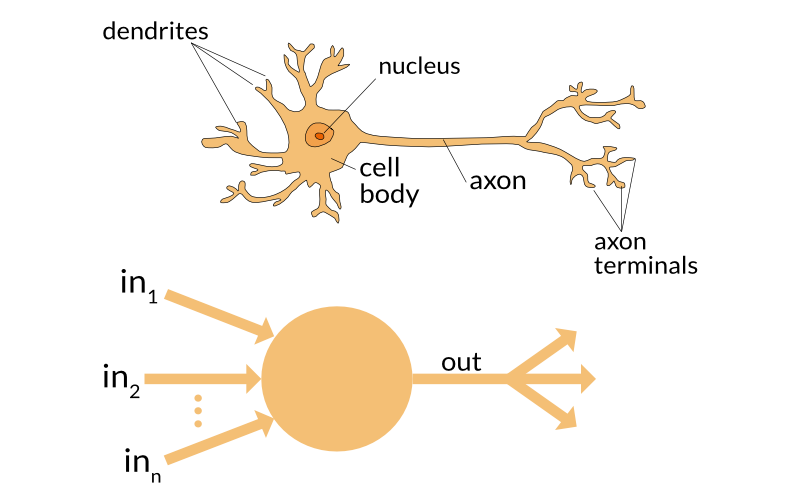
\includegraphics[width = 100mm]{images/neuron.png}
	\caption{Dalla rappresentazione biologica di un neurone al modello matematico.}
	\label{img:neurone}
\end{figure}

Questa attività biologica può essere rappresentata da un modello matematico nel quale i segnali che viaggiano attraverso gli assoni interagiscono con i dendriti dei neuroni con i quali sono collegati. La modifica delle sinapsi (i pesi $w$), rappresenta l'apprendimento. Nel modello base i dendriti portano il segnale al corpo della cellula, dove sono sommati: se il risultato di questa somma supera una certa soglia, il neurone attiva l'impulso attraverso l'assone. Tale somma viene attivata da una funzione di attivazione. In altre parole, ogni neurone esegue un prodotto vettoriale tra i suoi input e il suo set di pesi, somma un termine di distorsione (bias) e infine applica una funzione di attivazione non lineare. La funzione di attivazione deve necessariamente essere non lineare, in caso contrario la rete neurale si ridurrebbe ad un modello lineare generalizzato.

\begin{figure}[htb]
	\centering
	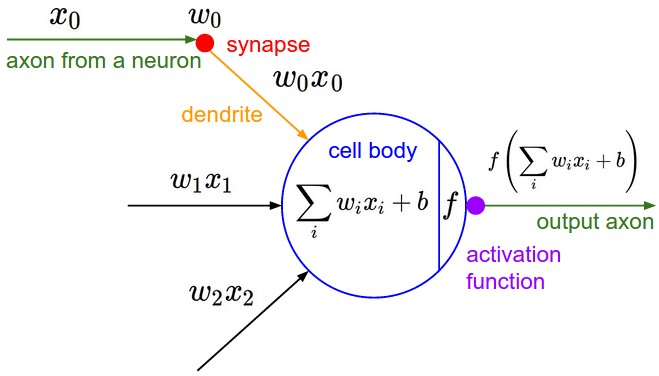
\includegraphics[width = 100mm]{images/neuron_model.jpeg}
	\caption{Modello matematico di neurone.}
	\label{img:modello_neurone}
\end{figure}

Nella figura è rappresentata una semplice rete neurale con 4 predittori $x_j$, un singolo strato nascosto composto da 5 neuroni calcolato: $x^{(1)} = \sigma(Wx^{(0)} + b)$ layer 1 dove $\sigma$ è la funzione di attivazione, $W$ è il set di pesi, $x^{(0)}$ è il vettore di input e $b$ è il bias. L'output è data da una singola unità $y = \sigma(Wx^{(1)} + b)$.

L'idea di base è quella che ogni neurone apprenda una semplice funzione binaria. Lo strato finale è caratterizzato anch'esso dalla presenza di un vettore di pesi e di una funzione di output, che generalmente corrisponde alla funzione identità in problemi di regressione, o alla softmax in problemi di classificazione. Cambiando il numero di strati e dei neuroni, le reti neurali possono essere considerate come approssimatori universali di funzioni \cite{hornik1989multilayer}.

\begin{figure}[htb]
	\centering
	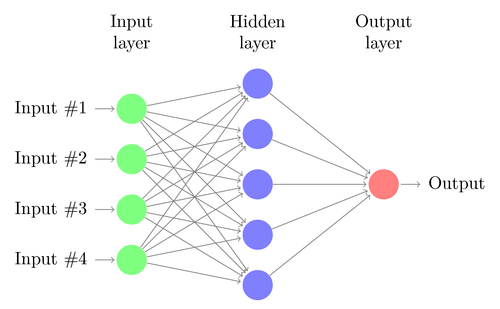
\includegraphics[width = 100mm]{images/onehidden.png}
	\caption{Multilayer perceptron.}
	\label{img:multilayer_perceptron}
\end{figure}

Il termine Deep Learning prende nome dalla profondità che caratterizza le reti neurali multistrato, dove con profondità ci si riferisce al numero di strati nascosti presenti. Le reti deep vengono infatti chiamate anche MLP, ovvero MultiLayer Perceptron \cite{goodfellow2016deep}.


\subsection{Layer}
I neuroni sono organizzati in layer, moduli di elaborazione dati che possono essere considerati come un filtro per i dati. Alcuni dati entrano, e ne escono in una forma più utile. Nello specifico, i layer estraggono rappresentazioni che, auspicabilmente, dovrebbero essere più significative per il problema in questione. La maggior parte dell'apprendimento consiste nel concatenare insieme semplici livelli che implementeranno una forma di astrazione progressiva dei dati, fino ad una rappresentazione di alto livello in grado di portare a termine il task.

\subsection{Activation function}
Lo scopo della funzione di attivazione è quello di aggiungere non-linearità nella rete, permettendo di modellare output che non variano linearmente al variare dei predittori. Questo significa che l'output non può essere rappresentato da una combinazione lineare dell'input. Senza non-linearità, anche aggiungendo diversi strati nascosti in una rete, questi risulterebbero equivalenti ad uno strato solo (single-layer Perceptron).

\subsubsection{Sigmoid}
Inizialmente la più utilizzata, la funzione sigmoide è stata progressivamente accantonata negli ultimi anni per via di alcune problematiche che comporta a livello pratico.

La prima e più importante è quella relativa alla dissolvenza del gradiente in seguito alla saturazione dei neuroni, ossia quei neuroni che presentano valori di output agli estremi del codominio della funzione di attivazione, in questo caso $(0, 1)$. Tale saturazione diventa problematica durante la fase di addestramento della rete (Back Propagation, sezione \ref{backprop}), in quanto il gradiente locale assume valori prossimi allo zero, conducendo così all'annullamento del gradiente globale \cite{glorot2010understanding}. In pratica si ha un flusso utile del gradiente solo per valori di input che rimangono all'interno di una zona di sicurezza, cioè nei dintorni dello zero.

Il secondo problema deriva invece dal fatto che gli output della funzione sigmoide non sono centrati intorno allo zero \cite{lecun1998gradient}. Si consideri il caso in cui tutti gli input di un nodo sono positivi. L'aggiornamento dei pesi entranti in un determinato neurone avviene in modo proporzionale all'errore in quel nodo (uno scalare) ed il vettore di input. Se tutte le componenti del vettore in input sono positive, tutti gli aggiornamenti dei pesi che arrivano in quel neurone avranno lo stesso segno (il segno dell'errore) e i pesi quindi saranno o tutti incrementati o tutti diminuiti. Se il vettore di pesi in considerazione deve cambiare direzione, questo può avvenire solamente dopo diverse iterazioni di aggiornamento (zigzagando), rallentando così l'apprendimento. Questo si comporta inoltre come una fonte di bias sistematico per i neuroni nello strato successivo della rete. Per aggirare questo problema è stata introdotta come funzione di attivazione la Tangente Iperbolica in quanto funzione dispari. L'apprendimento con Backpropagation con funzioni dispari porta ad una convergenza più veloce rispetto ad un processo con funzioni non simmetriche \cite{haykin2004comprehensive}.

Il terzo e ultimo difetto della funzione sigmoide è che l'operazione esponenziale al denominatore è molto costosa dal punto dal punto di vista computazionale, soprattutto rispetto alle alternative che verranno presentate di seguito.

\begin{figure}[htb]
	\centering
	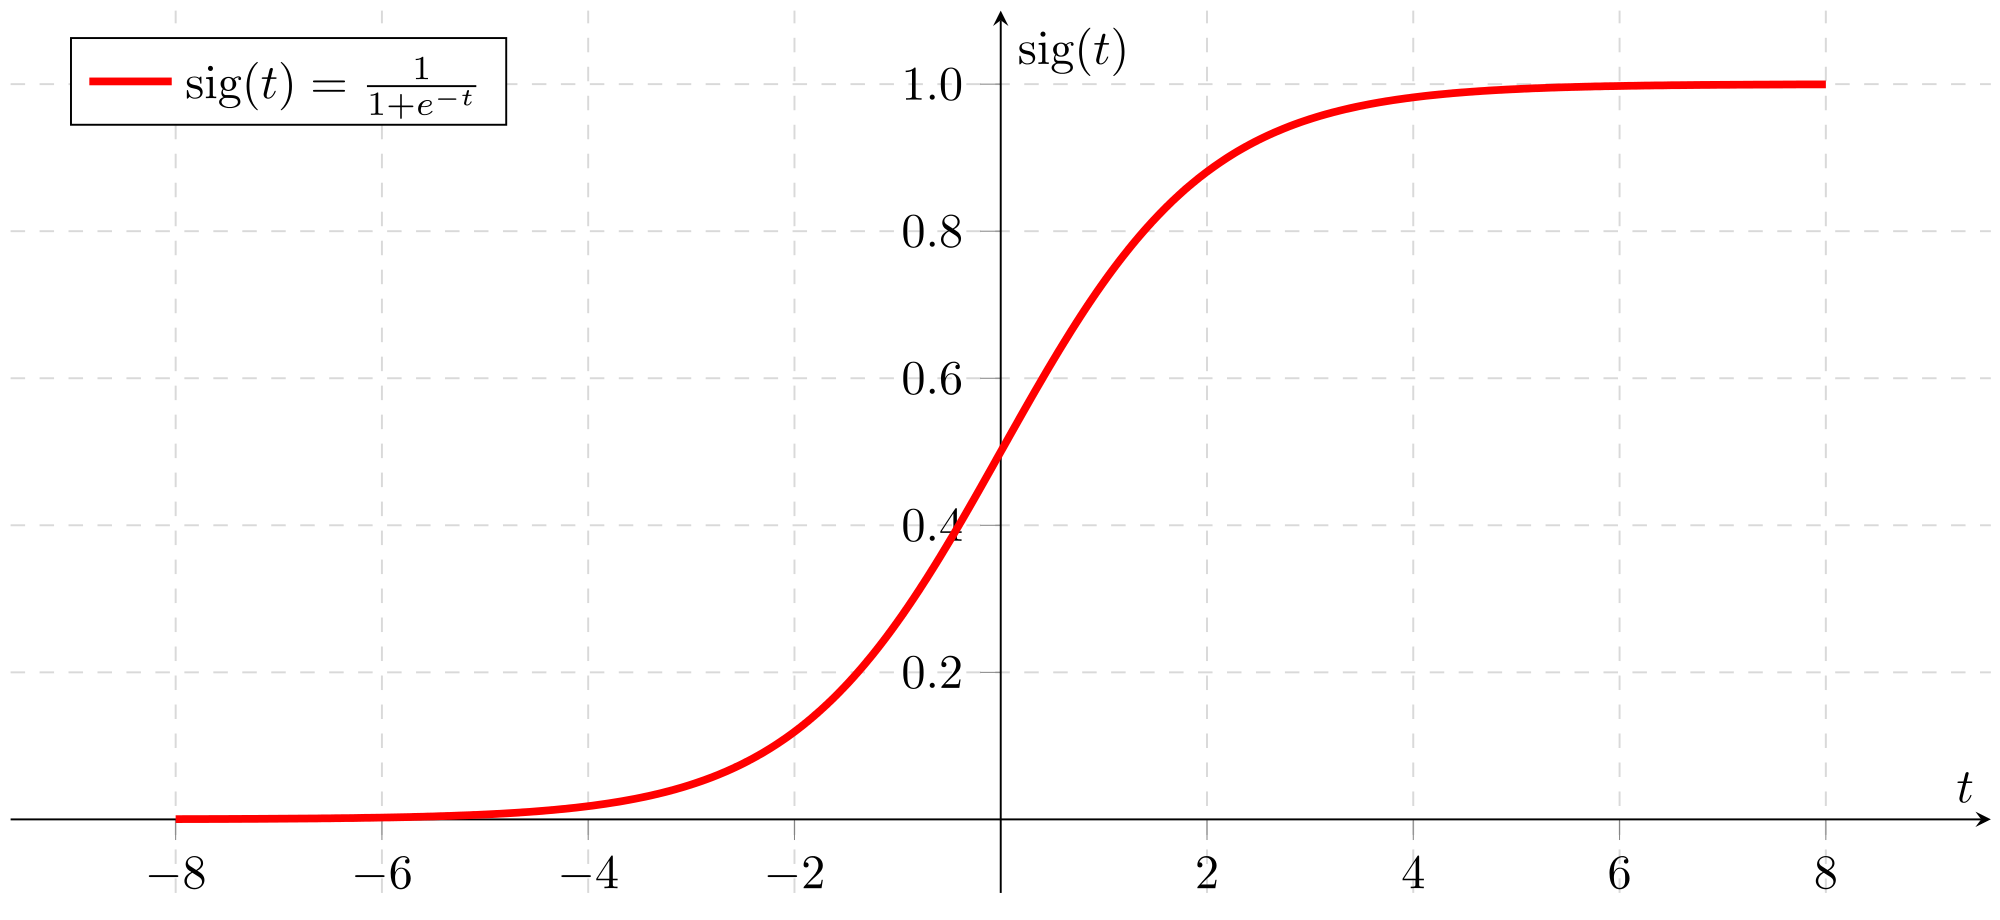
\includegraphics[width = 100mm]{images/sigmoid.png}
	\caption{Funzione sigmoide.}
	\label{img:sigmoid}
\end{figure}

\subsubsection{TanH}
Il problema degli output non centrati sullo zero \cite{haykin2004comprehensive} della sigmoide può essere risolto ricorrendo all'utilizzo della tangente iperbolica, la quale presenta codominio $(−1, 1)$ centrato sull'origine degli assi. Tuttavia, rimane il problema della saturazione dei neuroni, anzi viene addirittura accentuato, dal momento che la zona di sicurezza risulta ancora più ristretta.

\begin{figure}[htb]
	\centering
	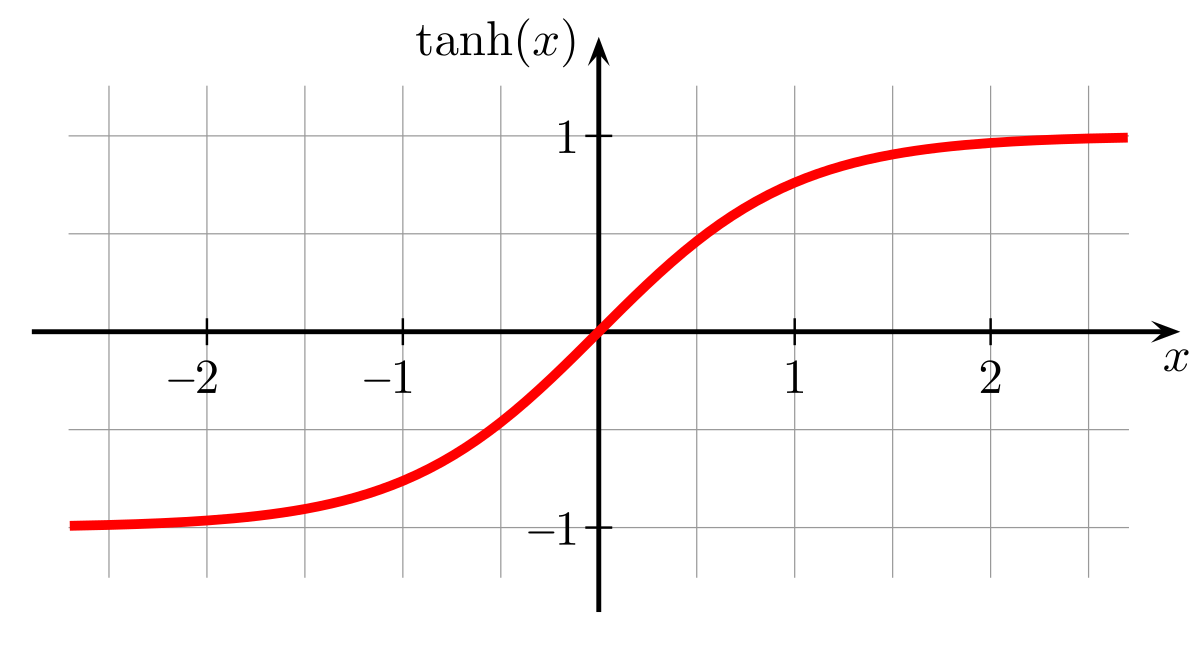
\includegraphics[width = 100mm]{images/tanh.png}
	\caption{Funzione TanH.}
	\label{img:tanh}
\end{figure}

\subsubsection{ReLU}
La Rectified Linear Unit (ReLU) è diventata popolare negli ultimi anni per via dell'incremento prestazionale che offre nel processo di convergenza: velocizza infatti di circa 6 volte la discesa del gradiente rispetto alle alternative viste finora. Questo risultato è da attribuire in larga parte al fatto che la ReLU risolve il problema della dissolvenza del gradiente \cite{glorot2010understanding}, non andando a saturare i neuroni. Durante la fase di Back Propagation (sezione \ref{backprop}) infatti, se il gradiente calcolato fino a quel punto è positivo questo viene semplicemente lasciato passare, perchè la derivata locale per il quale viene moltiplicato è pari ad uno. Eventuali problemi sorgono invece quando il gradiente accumulato ha segno negativo, in quanto questo viene azzerato (le derivata locale è nulla lungo tutto il semiasse negativo) con la conseguenza che i pesi non vengono aggiornati. Fortunatamente questo problema può essere alleviato attraverso l'utilizzo di un algoritmo SGD (batch size maggiori di 1) \cite{ioffe2015batch}: considerando più dati alla volta c'è infatti la speranza che non tutti gli input del batch provochino l'azzeramento del gradiente, tenendo così in vita il processo di apprendimento del neurone. Al contrario, se per ogni osservazione la ReLU riceve valori negativi, allora il neurone "muore", e non c'è speranza che i pesi vengano aggiornati. Valori elevati del learning rate amplificano questo problema, dal momento che cambiamenti più consistenti dei pesi si traducono in una maggiore probabilità che questi affondino nella "zona morta".
\begin{figure}[htb]
	\centering
	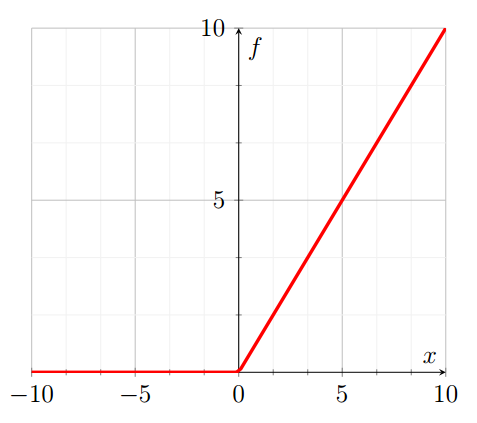
\includegraphics[width = 100mm]{images/relu.png}
	\caption{Funzione ReLU.}
	\label{img:relu}
\end{figure}

\subsection{Loss function}
A loss function: how the network will be able to measure its performance on the training data, and thus how it will be able to steer itself in the right direction.
\subsection{Optimizer}
An optimizer—The mechanism through which the network will update itself based on the data it sees and its loss function.
\subsection{Metrics}
Metrics to monitor during training and testing—Here, we’ll only care about accu- racy (the fraction of the images that were correctly classified).



\subsection{BackPropagation}
\label{backprop}
L'apprendimento dei pesi di una rete neurale non risulta un compito semplice, trattandosi come abbiamo visto di una complessa funzione gerarchica $f(x;W)$ del vettore di input $x$ e della collezione di pesi $W$.  Innanzitutto è necessario scegliere opportunamente le funzioni di attivazione in modo che tale funzione risulti differenziabile. Si tratta quindi di risolvere una funzione di perdita $L[y, f(x)]$.

Le funzioni di perdita sono generalmente convesse in $f$, ma non negli elementi di $W$, con la conseguenza che ci troviamo a dover risolvere un problema di minimizzazione su una superficie che presenta una grande quantità di minimi locali. Una soluzione è quella di effettuare più stime dello stesso modello con differenti inizializzazioni dei parametri, per scegliere infine quello che risulta essere migliore. Una procedura di questo tipo può però richiedere molto tempo, che spesso non è disponibile, pertanto generalmente ci si tende ad accontentare di buoni minimi locali.

I principali metodi utilizzati sono basati sulla tecnica della discesa del gradiente, la cui implementazione in questo contesto prende il nome di Back-Propagation \cite{werbos1974beyond}, in virtù del fatto che lo scarto registrato in corrispondenza di un certo dato viene fatto propagare all'indietro nella rete per ottenere le formule di aggiornamento dei coefficienti. Dal momento che $f(x;W)$ è definita come una composizione di funzioni a partire dai valori di input della rete, gli elementi di $W$ sono disponibili solo in successione (quella degli strati) e pertanto la differenziazione del gradiente seguirà la regola della catena (chain rule).

Data una generica osservazione $(x, y)$ l'algoritmo di back-propagation prevede di effettuare un primo passo in avanti lungo l'intera rete (feed-forward step) e salvare le attivazioni che si creano ad ogni nodo $x_{l}^{(k)}$ di ogni strato $l$, incluso quello di output. La responsabilità di ogni nodo nella previsione del vero valore di $y$ viene quindi misurata attraverso il calcolo di un termine d'errore $\delta_{l}^{(k)}$. Nel caso delle attivazioni terminali $x_{l}^{(k)}$ il calcolo di tali errori è semplice: coincide infatti con i residui o loro trasformazioni, in base a come viene definita la funzione di perdita. Per le attivazioni degli strati intermedi $\delta_{l}^{(k)}$ viene calcolato invece come somma pesata dei termini d'errore dei nodi che utilizzano $x_{l}^{(k)}$ come input.

Una volta calcolato il gradiente è possibile procedere con l'aggiornamento del sistema dei pesi. Il calcolo del gradiente ci fornisce la direzione lungo la quale la superficie da minimizzare è più ripida, ma nessuna informazione circa la lunghezza del passo che dovremmo compiere. Tale quantità viene denominata learning-rate e costituisce l'iperparametro più importante da regolare in una rete neurale: valori alti portano ad una convergenza più veloce ma sono rischiosi dal momento che potrebbero saltare il minimo ottimale o fluttuare intorno ad esso, mentre valori bassi sono responsabili di una convergenza lenta e possono comportare il blocco dell'algoritmo in un minimo locale non ottimale.

\subsection{Stochastic Gradient Descent}
Esistono alcune varianti dell'algoritmo di discesa del gradiente che differiscono nella quantità di dati utilizzati nel calcolo del gradiente prima di effettuare l'aggiornamento dei parametri. Quella classica utilizza ad ogni iterazione l'intero dataset. Tuttavia, può spesso risultare più efficiente processare piccole quantità di dati (batch) per volta, generalmente campionate in maniera casuale, da qui il nome Stochastic Gradient Descent (Bottou, 2010). Tale scelta è obbligata quando le dimensioni del dataset sono tali da non poter essere caricato in memoria. Valori estremi del batch come n oppure 1 possono causare problemi rispettivamente di calcoli ridondanti (il gradiente viene ricalcolato sempre su osservazioni simili prima dell'aggiornamento) e di fluttuazioni della funzione da minimizzare, a causa di aggiornamenti troppo frequenti e variabili, essendo basati sulla singola osservazione. Di conseguenza si tendono a scegliere valori intermedi. Indipendentemente dal numero di iterazioni e dalla dimensione del batch prescelta, ogni volta che tutte le osservazioni del dataset vengono utilizzate per il calcolo del gradiente si dice che viene completata un'epoca.

\subsection{Ottimizzazione discesa del Gradiente}
Ci sono alcune modifiche che possono essere apportate all'algoritmo di discesa del gradiente per migliorarne le performance, legate soprattutto al learning rate. Possono sorgere complicazioni invece quando si tratta di minimizzare funzione non convesse, con il rischio di rimanere intrappolati in minimi locali non ottimali. Di seguito verranno presentati alcuni algoritmi di ottimizzazione che mirano alla risoluzione di questo tipo di problematiche.

\begin{itemize}
    \item \textbf{Momentum}: SGD presenta alcune difficoltà in prossimità di aree dove la superficie presenta una curvatura molto più accentuata in una direzione rispetto all'altra (Sutton, 1986). In questo scenario infatti l'algoritmo tende ad oscillare lungo il versante più ripido, rallentando così la convergenza verso il minimo locale ottimale. Momentum \cite{qian1999momentum} è un metodo che aiuta ad accelerare la discesa del gradiente verso la direzione corretta, smorzando l'effetto indotto dalle oscillazioni. Tale risultato si ottiene aggiungendo al termine di aggiornamento corrente una frazione gamma del vettore di aggiornamento precedente.
    
    \item \textbf{AdaGrad}: Momentum permette di adattare i nostri aggiornamenti in relazione alla superficie da minimizzare velocizzando così la convergenza, ma non fa nessuna distinzione circa l'importanza dei parametri, trattandoli tutti allo stesso modo. Adagrad \cite{duchi2011adaptive} è un algoritmo di ottimizzazione nato proprio con questo scopo: adattare il learning rate ai parametri, permettendo così di effettuare aggiornamenti più consistenti in corrispondenza dei parametri relativi alle features meno frequenti, e viceversa. In particolare, nella sua regola di aggiornamento, Adagrad utilizza un alpha differente per ogni parametro ad ogni iterazione, modificando quest'ultimo sulla base dei gradienti passati che sono stati calcolati per lo specifico parametro. Uno dei più grandi benefici di Adagrad consiste nell'eliminare la necessità di settare manualmente il learning rate: è necessario impostare solamente il valore iniziale. D'altra parte, il suo punto debole è invece l'accumulo eccessivo del quadrato dei gradienti al denominatore, che comporta un'esagerata e progressiva riduzione del learning rate, il quale tende a diventare infinitamente piccolo, al punto tale che l'algoritmo non è più in grado di acquisire nuova informazione, arrestando così il processo di convergenza.
\end{itemize}

























Spiegato il framework di base nel quale il Deep Learning rientra, nella prossima sezione parleremo delle reti Convolutional, le quali introducono un nuovo tipo di layer, più adatto all'elaborazione delle immagini in quanto in grado di imparare pattern locali invece di pattern globali.

\section{Convolutional Neural Networks}

\section{Computer Vision}

\subsection{Image Classification}

% just a reminder it's not a task
\subsection{Class Activation Map}

\subsection{Object detection}

\subsection{Semantic Segmentation}

\chapter{State of the Art}
\label{cap:chapter2}
% !TEX encoding = UTF-8
% !TEX TS-program = pdflatex
% !TEX root = ../Tesi.tex

%************************************************

%************************************************

\section{State of the Art}

\begin{figure}[htb]
	\centering
	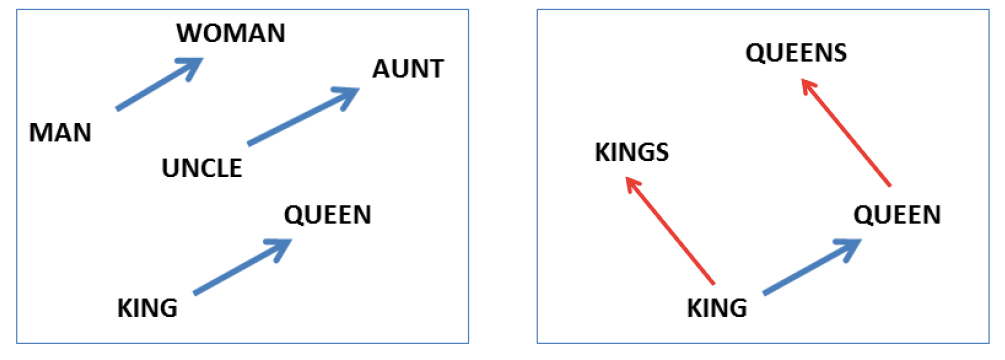
\includegraphics[width = 100mm]{images/king-queen.png}
	\caption{Vettori corrispondenti alle parole}
	\label{2w2v}
\end{figure}

\chapter{Pipeline}
\label{cap:chapter3}
% !TEX encoding = UTF-8
% !TEX TS-program = pdflatex
% !TEX root = ../Tesi.tex
% !TEX spellcheck = it-IT

%************************************************

%************************************************

\section{Datasets}

\subsection{Exploration}

\begin{itemize}
    \item \% auto VS rest 2 FTE
    \item Exploration Dataset 2 FTE
    \item \% noise 4 FTE
    \item Black Box 2 FTE
\end{itemize}

\section{Car Detection / No Car}

\begin{itemize}
    \item DATA: Stanford Car - Open Images - Kaggle Carvana - Label Me
    \item INPUT: Images
    \item OUTPUT: Cropped Bounding Boxes with cars
\end{itemize}

\section{Car Part Segmentation}
\begin{itemize}
    \item DATA: PASCAL-part
    \item INPUT: Car images
    \item OUTPUT: Car parts images
\end{itemize}

\section{Damage / No Damage}

\begin{itemize}
    \item DATA: My Car History Assistant - Wrecked Exotics - Neokt - Manually Crafted
    \item INPUT: Car images OR Car parts images
    \item OUTPUT: Class in damage, no damage for each image
\end{itemize}


\section{Repair / replace}

\begin{itemize}
    \item DATA: Neokt - ?
    \item INPUT: Parts Images, Parts classes, Data about the car
    \item OUTPUT: Class in repair, replace for each part OR class in no damage, repair, replace
\end{itemize}

\chapter{Evaluation}
\label{cap:chapter4}
% !TEX encoding = UTF-8
% !TEX TS-program = pdflatex
% !TEX root = ../Tesi.tex
% !TEX spellcheck = it-IT

%************************************************

%************************************************

\section{Performance table}
ciao

\cite{patil2017deep}

\cite{liu2017monza}

\cite{liu2018deep}

\cite{guo2018review}

\cite{he2017mask}

\cite{chahal2018survey}

\cite{xie2018bag}

% \chapter{Critical analysis}
\chapter{Conclusion}
\label{cap:conclusion}
% !TEX encoding = UTF-8
% !TEX TS-program = pdflatex
% !TEX root = ../Tesi.tex
% !TEX spellcheck = it-IT

%************************************************
% Conclusione
%************************************************

\section{ProvaC}


% \chapter{Critical analysis}
% \input{Capitoli/Conclusioni}


\bibliographystyle{plain}
\bibliography{Bibliography}

\end{document}
